\documentclass[11pt,a4paper,UTF8]{ctexart}

\usepackage[a4paper,margin=20mm,headheight=15pt]{geometry}
\usepackage{booktabs,tabularx,longtable,array,multirow}
\usepackage{xcolor,colortbl}
\usepackage{tikz}
\usetikzlibrary{arrows.meta,positioning,fit,shapes.geometric,calc}
\usepackage{hyperref}
\usepackage{enumitem}
\usepackage{fancyhdr,lastpage}
\usepackage{microtype}
\usepackage{amsmath,amssymb}
\usepackage{listings}

\definecolor{navy}{HTML}{153B5B}
\definecolor{blue}{HTML}{2E6F9E}
\definecolor{green}{HTML}{2E7D5B}
\definecolor{amber}{HTML}{B97910}
\definecolor{red}{HTML}{A23B3B}
\definecolor{ink}{HTML}{263238}
\definecolor{muted}{HTML}{607D8B}
\definecolor{paleBlue}{HTML}{EAF3F8}
\definecolor{paleGreen}{HTML}{EAF5EF}
\definecolor{paleAmber}{HTML}{FFF5DF}
\definecolor{paleRed}{HTML}{FCECEC}
\definecolor{linegray}{HTML}{D7E0E5}

\hypersetup{
  colorlinks=true,
  linkcolor=navy,
  urlcolor=blue,
  pdftitle={FreeRTOS V6.1.1 Scheduler 通用形式化验证进展报告},
  pdfauthor={Codex with external Pro review},
  pdfsubject={Isabelle/HOL universal scheduler refinement progress, 2026-08-11}
}

\pagestyle{fancy}
\fancyhf{}
\fancyhead[L]{\small FreeRTOS V6.1.1 Scheduler 通用验证}
\fancyhead[R]{\small 进展审计 · 2026-08-11}
\fancyfoot[C]{\small \thepage~/~\pageref{LastPage}}
\renewcommand{\headrulewidth}{0.4pt}

\setlist[itemize]{leftmargin=1.7em,itemsep=0.35em,topsep=0.45em}
\setlist[enumerate]{leftmargin=1.9em,itemsep=0.4em,topsep=0.45em}
\renewcommand{\arraystretch}{1.25}
\setlength{\emergencystretch}{2.5em}
\newcolumntype{Y}{>{\raggedright\arraybackslash}X}
\newcolumntype{C}[1]{>{\centering\arraybackslash}p{#1}}

\newcommand{\checked}{\colorbox{paleGreen}{\textcolor{green}{\textbf{C · checked}}}}
\newcommand{\repoev}{\colorbox{paleBlue}{\textcolor{blue}{\textbf{R · repository}}}}
\newcommand{\audit}{\colorbox{paleAmber}{\textcolor{amber}{\textbf{A · audited}}}}
\newcommand{\recommend}{\colorbox{paleRed}{\textcolor{red}{\textbf{N · next}}}}
\newcommand{\code}[1]{\nolinkurl{#1}}
\newcommand{\claimbox}[2]{%
  \par\medskip\noindent
  \fcolorbox{#1}{white}{\begin{minipage}{0.94\linewidth}#2\end{minipage}}
  \par\medskip
}

\begin{document}

% --------------------------------------------------------------------------
% Page 1: cover
% --------------------------------------------------------------------------
\begin{titlepage}
  \centering
  \vspace*{18mm}
  {\color{navy}\rule{\textwidth}{1.4pt}}\\[14mm]
  {\fontsize{25}{32}\selectfont\bfseries\color{navy}
   FreeRTOS V6.1.1 Scheduler\\[2mm]
   通用形式化验证进展报告}\\[8mm]
  {\Large Isabelle/HOL · generated C source · cursor-general semantics}\\[16mm]

  \begin{tikzpicture}
    \node[draw=navy,rounded corners=3pt,fill=paleBlue,
          minimum width=0.82\textwidth,minimum height=34mm,align=center] {
      {\fontsize{30}{34}\selectfont\bfseries\color{navy}严格闭环约 35--40\%}\\[2mm]
      {\large 粗粒度 gate 台账：暂定 $9/20=45\%$}\\[1mm]
      {\small 两个口径必须分开；均不是 theory/session 数量比}
    };
  \end{tikzpicture}

  \vfill
  \begin{tabular}{rl}
    报告日期：& 2026-08-11\\
    基线提交：& \code{1663ad0}\\
    分支：& \code{agent/universal-scheduler-refinement}\\
    公开审阅：& \url{https://github.com/hellotommmy/freertos-v611-scheduler-isabelle/pull/2}\\
    核验准则：& Isabelle2025-2，\code{quick_and_dirty=false}，无承认性证明\\
  \end{tabular}

  \vfill
  {\color{navy}\rule{\textwidth}{1.4pt}}\\[4mm]
  {\small 本报告严格区分：\checked\quad \repoev\quad \audit\quad \recommend}
\end{titlepage}

% --------------------------------------------------------------------------
% Page 2: executive summary
% --------------------------------------------------------------------------
\section{结论先行：已经完成多少？}

\claimbox{navy}{
\textbf{审慎结论。}若目标是旧的 fixed-witness / sealed milestone，则它已经完成；
若目标是当前声明的“所有合法输入、任意合法 cursor、managed 与 runnable 分离、五根
generated-source 混合 trace、并发契约分离”的更强目标，则需要同时给出两种读数：
\textbf{严格 acceptance closure 约 35--40\%}；若只衡量已经可复用的表示、due-loop 与
tick 证明基础设施，则为\textbf{约 45--50\%}。另按外部 Pro 建议的粗粒度
$20$-gate 台账可暂记为 $9/20=45\%$，但其中 A1--A8 尚须在仓库内逐项命名，且
\code{xTaskGetTickCount} 只能按 root-local 功能结果计分，不能冒充完整 common scheduler
framing。上述数字都是审计口径，不是 Isabelle 定理，也不是把 371 个 theory 或 311 个
session 逐个计数所得。
}

\subsection{为何不能按 theory/session 数量计算}

\begin{itemize}
  \item 一个 session 可能只证明一个 selector frame，也可能关闭一个 arbitrary-list
        generated while；二者语义权重不相等。\audit
  \item 同一语义缺口常被拆成多个小 session 以避免 Isabelle 搜索爆炸；拆分会增加文件数，
        却不会自动提高覆盖率。\repoev
  \item “某个分支 checker-green”不等于“该根函数所有合法输入 checker-green”。例如
        suspended-only switch、zero-delay 和固定 P2 delay 都是有效结果，但不应计成通用闭环。\checked
  \item 最终目标的负载门槛是：通用表示关系、每个根函数的 all-branch public closure、
        共用边界、混合有限 trace，以及与 generated source 相连的并发契约。\audit
\end{itemize}

\subsection{两个同时成立的进度视角}

\noindent\begin{tabularx}{\textwidth}{p{0.23\textwidth}Y C{22mm} Y}
\toprule
视角 & 已获得的强证据 & 读数 & 解释\\
\midrule
基础设施/单根深度 & cursor-general 强快照、managed-domain due loop、完整 tick pipeline、公共边界、有限 tick trace
& 约 45--50\% & 大量最难的表示与 tick 控制流已闭合\\
粗粒度 20-gate 台账 & 暂按 A 6/8、B 2/5、C 0/4、D 1/3 汇总；A1--A8 名称仍待固化
& $9/20=45\%$ & 可复算的暂定工程台账；不是 kernel 输出，也不是严格 closure 百分比\\
最终 acceptance gates & 五根中只有 tick 与 tick-read 接近通用公共闭包；mixed trace 与 generated concurrency 仍开放
& 约 35--40\% & 只有 tick 具有完整 common scheduler framing；tick-read 仍需 framing adapter\\
\bottomrule
\end{tabularx}

\noindent 三个读数回答不同问题，不应再合成一个看似精确的小数。“45--47\%”只可作为
带公开分母的 engineering-progress 台账或敏感性区间；对外回答“全部形式化证明完成多少”时，
应优先使用 35--40\% 的严格闭环区间，并同时列出门槛表。若第三方复算 45\%，必须先把
A1--A8 逐项命名，并明确 tick-read 的 framing 缺口。\audit

\medskip

% --------------------------------------------------------------------------
% Page 3: semantic gates and DAG
% --------------------------------------------------------------------------
\section{证明架构与语义门槛}

\begin{center}
\begin{tikzpicture}[
  node distance=8mm and 8mm,
  box/.style={draw,rounded corners=2pt,align=center,minimum height=9mm,
              text width=31mm,font=\small},
  done/.style={box,fill=paleGreen,draw=green},
  partial/.style={box,fill=paleAmber,draw=amber},
  open/.style={box,fill=paleRed,draw=red},
  edge/.style={-{Latex[length=2.2mm]},thick,draw=muted}
]
  \node[done] (src) {CParser / AutoCorres2\\generated semantics};
  \node[done,right=of src] (list) {通用 xLIST\\表示与操作};
  \node[done,right=of list] (snap) {cursor-general\\managed snapshot};

  \node[done,below=of list] (due) {one-due exact step\\family/role frame};
  \node[done,right=of due] (while) {任意 due-prefix\\while / finally};
  \node[done,right=of while] (tick) {generated tick\\all arithmetic classes};

  \node[done,below=of while] (pub) {public boundary\\re-entry};
  \node[done,right=of pub] (trace) {任意有限\\tick-only trace};
  \node[partial,left=of pub] (resume) {nested-critical\\Resume replay};

  \node[open,below=of pub] (roots) {其余三根\\universal closure};
  \node[open,left=of roots] (mixed) {五根 mixed\\finite trace};
  \node[open,right=of roots] (conc) {generated-source\\concurrency};

  \draw[edge] (src)--(list);
  \draw[edge] (list)--(snap);
  \draw[edge] (list)--(due);
  \draw[edge] (snap)--(due);
  \draw[edge] (due)--(while);
  \draw[edge] (while)--(tick);
  \draw[edge] (tick)--(pub);
  \draw[edge] (pub)--(trace);
  \draw[edge,dashed] (pub)--(resume);
  \draw[edge,dashed] (resume)--(roots);
  \draw[edge,dashed] (roots)--(mixed);
  \draw[edge,dashed] (roots)--(conc);
\end{tikzpicture}

\small 图 1：theorem/coverage DAG。绿色为 checker-green 类别，黄色为当前接缝，红色为未闭合 acceptance gate。
\end{center}

\subsection{门槛表}

\noindent\begin{tabularx}{\textwidth}{C{10mm}Y C{22mm} Y}
\toprule
门槛 & 定义 & 当前读数 & 解释\\
\midrule
A & list primitives、byte geometry、family coverage、cursor-general 表示 & 6/8（75\%） & 通用基础强，但不是完整 API closure\\
B & 冻结五根函数的 all-branch public refinement & 2/5 局部；1/5 完整 framing & tick 完整；tick-read 的返回值正确但 relation 尚未携带 full scheduler state\\
C & 共用 public invariant、五根 alphabet、mixed finite trace、跨根 closure & 0/4 & 已有 tick-only seed，不等于五根 gate 完成\\
D & concurrent abstract interface、modular environment、generated connection & 1/3 & 有基础设施；generated end-to-end 仍为 0\\
E & scope、工具链、QAD、排除项纪律 & 13/13 边界遵守 & 它是可信度条件，不计入证明覆盖率\\
\bottomrule
\end{tabularx}

\claimbox{amber}{
\audit\quad 任何百分比都不应由上表直接做算术平均。A--D 的依赖、难度和 acceptance
含义不同；最诚实的呈现是“区间 + 离散门槛表 + 逐根状态”，而不是单一精确小数。
}

\clearpage

% --------------------------------------------------------------------------
% Page 4: checked results
% --------------------------------------------------------------------------
\section{当前最关键的 checker-green 结果}

以下每项均指结果类别；只有仓库中实际存在且有绿色 session 证据的内容才标为
\checked。未注册的 nested-tick probes 不在本页。

\begin{enumerate}
  \item \textbf{通用 xLIST 与 raw/abstract 对齐。}任意合法 ring、节点、cursor、key 和
        byte-heap 几何下，删除、尾插、relabel、owner/container/key frame 具有精确关系。
        这些引理不固定任务身份或列表长度。\checked
  \item \textbf{Generic/Event 全根 family coverage。}ready、delayed A/B、suspended、
        termination、pending 与任意有限 external Event roots 被统一量化；cross-family storage
        separation 在同一 heap cutpoint 重建。\checked
  \item \textbf{managed $M$ 与 runnable $L$ 分离。}允许 termination 中存在 retired task，
        维持 $L\subseteq M$，避免旧 Gate-H 把 decoder carrier 错缩为 live set。\checked
  \item \textbf{phase-aware due-loop invariant。}非空 due head 不再错误要求 stable
        \code{core_wf/time_wf}；due phase 允许 $key\le now$，terminal 才恢复 stable snapshot。\checked
  \item \textbf{一个 due task 的 exact generated step。}从真实 generated body 得到 exact
        Result pointer、精确最终 globals、family/role/observation/scalar/current/boundary frames，
        并进入统一 successor witness。\checked
  \item \textbf{任意有限 due-prefix while/finally。}覆盖零 due、singleton、任意 all-due、
        due+future；future head 的 body 为 exception，empty 为 \code{Result NULL}，finally
        统一归一为 \code{Result ()}。\checked
  \item \textbf{32-bit modular tick。}suspended missed counter 的
        \code{MAX_WORD -> 0} 被保留；unlocked wrap 只在 literal signed guard 有定义时成功，
        signed-overflow 分支被证明无 successful run，而不是被 no-wrap 假设排除。\checked
  \item \textbf{cursor-general generated tick pipeline。}任意合法 delayed-list cursor、任意
        managed/termination/external families 下，从 generated prefix 经 arbitrary managed due loop
        得到完整 cursor-general endpoint。\checked
  \item \textbf{调用方隐藏 witness 的 public tick 边界闭包。}
        \begin{center}\footnotesize\ttfamily
          CursorGeneralStrongScheduler\\[-1mm]PublicBoundaryRel
        \end{center}
        该 relation 对调用方隐藏内部 witness 参数，并证明成功 tick
        重新建立同一 settled/unmasked public boundary。\checked
  \item \textbf{任意有限 repeated tick trace。}
        \code{cursor_general_vTaskIncrementTick_finite_trace} 对任意 $n$、任意满足稳定性和逐步
        arithmetic-enabled 的调用者关系，给出 $n$ 次
        \code{task_increment_tick_modular_abs} 的精确迭代态。\checked
\end{enumerate}

\clearpage

% --------------------------------------------------------------------------
% Page 5: root coverage
% --------------------------------------------------------------------------
\section{冻结五根函数的真实覆盖状态}

{\small
\noindent\begin{tabularx}{\textwidth}{p{31mm}p{34mm}Y p{22mm}}
\toprule
根函数 & 最高已核验结果 & 仍缺什么 & 状态\\
\midrule
{\scriptsize\code{xTaskGetTickCount}} & quiescent tick/depth/mask relation 下的返回值 refinement & full scheduler frame 与 common five-root boundary adapter & \cellcolor{paleGreen}局部完整\\
{\scriptsize\code{vTaskIncrementTick}} & cursor-general public closure、all-arithmetic classification、finite tick trace & nested Resume replay 与 mixed-call composition & \cellcolor{paleGreen}单根很强\\
{\scriptsize\code{vTaskSwitchContext}} & suspended-only refinement & unlocked ready selection、任意 ready cursor、public re-entry & \cellcolor{paleAmber}部分\\
{\scriptsize\code{vTaskDelay}} & zero-delay 分支；固定 artifact-bound P2 positive delay 2 & 任意 delay/priority/task、blocking list migration、public closure & \cellcolor{paleAmber}部分\\
{\scriptsize\code{vTaskDelayUntil}} & suspended/no-delay 分支 & blocking 与 nonblocking all branches、wrap、public closure & \cellcolor{paleAmber}部分\\
\bottomrule
\end{tabularx}
}

\subsection{为什么“2/5”仍需谨慎}

\begin{itemize}
  \item tick-read 的控制流简单，而且当前 relation 只携带 tick/depth/mask；返回值证明完整，
        但尚不能直接作为 full scheduler public framing 的一根 closure。
  \item tick 的单根有限 trace 已经是真正通用的重要 milestone，但 mixed trace 尚不存在，
        因而不能把它描述成“scheduler trace correctness”。
  \item fixed P2 delay 证明的是一个 artifact-specialised witness，价值在于 generated-source
        inhabitation，而不在于覆盖 arbitrary delay input。
\end{itemize}

\subsection{机器证据摘要}

{\small
\noindent\begin{tabularx}{\textwidth}{p{49mm}p{18mm}p{18mm}Y}
\toprule
Run & Exit/QAD & 总耗时 & 支撑结论\\
\midrule
\shortstack[l]{\scriptsize\ttfamily 20260811Tcursor-general\\[-1mm]\scriptsize\ttfamily -tick-boundary-02} & 0 / false & 249.268 s & public tick boundary closure\\
\shortstack[l]{\scriptsize\ttfamily 20260811Tcursor-general\\[-1mm]\scriptsize\ttfamily -tick-trace-08} & 0 / false & 261.430 s & arbitrary finite tick-only trace\\
\shortstack[l]{\scriptsize\ttfamily 20260731Tscheduler-tick\\[-1mm]\scriptsize\ttfamily -refine-03-explicit-model-op} & 0 / false & 24.323 s & xTaskGetTickCount refinement\\
\shortstack[l]{\scriptsize\ttfamily 20260803Tscheduler-delay\\[-1mm]\scriptsize\ttfamily -zero-03-mod-yield} & 0 / false & 16.508 s & zero-delay modular-yield branch\\
\bottomrule
\end{tabularx}
}

\noindent\repoev\quad Git 基线为 \code{1663ad0}，准备报告时与 upstream 为 0 ahead / 0 behind。

\clearpage

% --------------------------------------------------------------------------
% Page 6: Resume trace
% --------------------------------------------------------------------------
\section{当前关键接缝：xTaskResumeAll 的 nested-critical replay}

\begin{center}
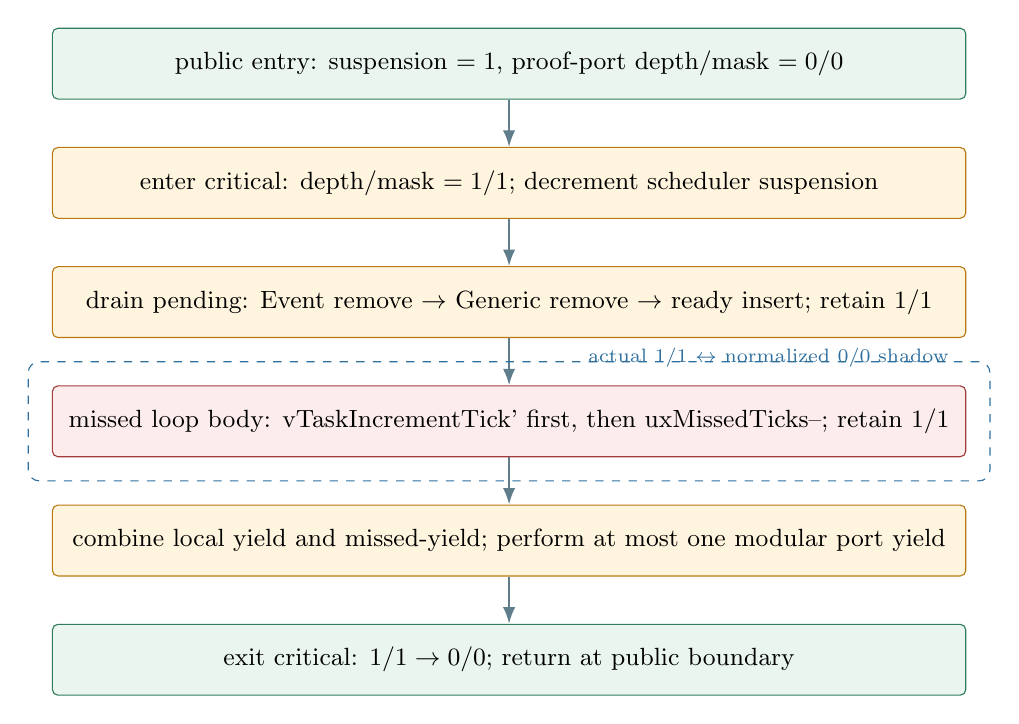
\begin{tikzpicture}[
  node distance=6mm,
  cut/.style={draw,rounded corners=2pt,minimum width=116mm,minimum height=9mm,
              align=left,font=\small},
  pub/.style={cut,fill=paleGreen,draw=green},
  inner/.style={cut,fill=paleAmber,draw=amber},
  danger/.style={cut,fill=paleRed,draw=red},
  arr/.style={-{Latex[length=2.1mm]},thick,draw=muted}
]
  \node[pub] (p0) {public entry: suspension $=1$, proof-port depth/mask $=0/0$};
  \node[inner,below=of p0] (p1) {enter critical: depth/mask $=1/1$; decrement scheduler suspension};
  \node[inner,below=of p1] (p2) {drain pending: Event remove $\to$ Generic remove $\to$ ready insert; retain $1/1$};
  \node[danger,below=of p2] (p3) {missed loop body: \code{vTaskIncrementTick'} first, then \code{uxMissedTicks--}; retain $1/1$};
  \node[inner,below=of p3] (p4) {combine local yield and missed-yield; perform at most one modular port yield};
  \node[pub,below=of p4] (p5) {exit critical: $1/1\to0/0$; return at public boundary};
  \draw[arr] (p0)--(p1); \draw[arr] (p1)--(p2); \draw[arr] (p2)--(p3);
  \draw[arr] (p3)--(p4); \draw[arr] (p4)--(p5);
  \node[draw=blue,dashed,rounded corners,fit=(p3),inner sep=3mm] {};
  \node[blue,font=\scriptsize,anchor=south east]
        at ($(p3.north east)+(-1mm,1mm)$)
        {actual 1/1 $\leftrightarrow$ normalized 0/0 shadow};
\end{tikzpicture}

\small 图 2：source-order cutpoint 图。红色步骤不能直接套用 public-boundary tick theorem。
\end{center}

\subsection{推荐的语义桥}

定义只覆盖 proof-port 两个字段的函数 overlay：
\[
  \operatorname{overlay}_{d,m}(c_0)
  = c_0[\operatorname{critical\_depth}:=d,
        \operatorname{interrupts\_disabled}:=m].
\]
需要的是 generated tick 对这个函数图关系的 \emph{semantic self-bisimulation}：
\[
  \operatorname{rel\_spec\_monad}
  (c=\operatorname{overlay}_{d,m}(c_0))\ (=)\ tick'\ tick'.
\]
它允许把 normalized shadow 的 checker-green run 迁移到真实 nested state，并证明输出仍是同一个
overlay。仅有 modifies/frame theorem 不够，因为“不写这两个字段”并不推出“从不读取或据此分支”。
\audit

\claimbox{red}{
\textbf{当前状态：}两份 unregistered/unbuilt static probe 已把问题缩小到
\code{one_due_tick_unlocked_source} 的 overlay bisimulation；它们不是 checker-green 结果，
不计入完成率。下一 session 应先检查较小的 209 行 rel-spec probe，并最终合并 vocabulary。
}

\clearpage

% --------------------------------------------------------------------------
% Page 7: real gates
% --------------------------------------------------------------------------
\section{开放 gate 与反例}

\begin{longtable}{p{31mm}p{55mm}p{66mm}}
\toprule
开放 gate & 最小反例/原因 & Acceptance criterion\\
\midrule
\endhead
Nested/public mismatch & replay 位于 depth/mask $=1/1$；public relation 固定 $0/0$ & generated tick 的 overlay self-bisimulation 与 exact port frame checker-green\\
\addlinespace
Replay arithmetic horizon & tick=\code{0xFFFFFFFE}、overflow=\code{INT_MAX}、debt=2；第一步成功，第二步 wrap guard failure & 对每个剩余 replay index 的 safety invariant，以及首个 unsafe step 的 no-success theorem\\
\addlinespace
Pending port frame & 现有 pending body exact state保留端口值，但 loop/outer continuation 弱化后丢失 & 任意 pending 长度后仍精确保留 running/depth/mask，并传给 missed-loop continuation\\
\addlinespace
Managed Resume gate & 旧 gate 使用 live-domain 与 live task count；termination retired task 需要 managed-domain & pending task 仍 live，同时 family、observation、count、termination 和 external roots 全部以 managed 量化\\
\addlinespace
Modular yield count & concrete word \code{MAX_WORD+1=0}，旧 abstract nat \code{Suc MAX} 不相等 & modular-yield scalar relation经过 final yield和 public re-entry保持\\
\addlinespace
Universal delay & zero branch和固定 P2 delay 不能覆盖任意 delay/task/priority & arbitrary positive delay 的 exact generated state、list migration、yield与 public closure\\
\addlinespace
Universal switch & suspended-only theorem不覆盖 unlocked selection和 ready cursor推进 & all-branch switch theorem重建同一 common public boundary\\
\addlinespace
Five-root trace & tick-only trace没有 mixed alphabet & 五种 operation 的统一 step relation与任意 finite enabled sequence induction\\
\addlinespace
Generated concurrency & 旧 pure concurrent EnvTick 使用 nat Suc，且没有 generated-C connection & cursor-general modular environment、linearisation cutpoint、generated source realization分别 checker-green\\
\bottomrule
\end{longtable}

\subsection{这些为何不是“proof engineering 小修”}

每一项都存在合法输入反例，或当前 relation 明确丢失源码可观察状态。扩大 timeout、增加 simp、
把后态作为前提、固定 cursor、令 managed=live、添加 no-wrap，均不能消除这些语义反例。
它们要求改变 invariant、关系 carrier 或 theorem statement，然后再进行小步机器检查。\audit

\clearpage

% --------------------------------------------------------------------------
% Page 8: next session
% --------------------------------------------------------------------------
\section{下一 session 的严格执行顺序}

{\small
\noindent\begin{tabularx}{\textwidth}{C{8mm}p{34mm}Y Y}
\toprule
序 & 小 session / rung & Acceptance criterion & 首错 fallback\\
\midrule
1 & Overlay algebra & selector、graph relation、run-image iff、combinator closure 全绿 & 只注册 209 行 probe；按 command 二分，不增大 timeout\\
2 & Unlocked self-bisim & list remove/insert、due while、terminal/future 对 overlay commute & 先分别证明 callees；必要时为 while 建独立 child\\
3 & Protected tick & 实际 depth/mask 原样保留，抽象后态为 modular tick，protected entry 重建 & 用 rel-spec refinement 的定向 runs-to 迁移\\
4 & Missed body & 正 debt、unlocked、tick 后 decrement，exact \code{resume_missed_source_step_abs} & 分离 word predecessor 与 snapshot frame，小 theorem 先绿\\
5 & Missed loop & horizon-safe 成功 replay + first-unsafe no-success；steps 等同 replay abstraction & 对 debt 归纳；首个 bad index 作最小 witness\\
6 & Pending port frame & 任意 pending drain 后仍为真实 $1/1$，continuation获得 frame & 用 exact body state + list induction；不重跑大 VCG\\
7 & Managed Resume gate & retired、termination、external roots 与 cursors 保留；pending 任务仍属于 live & 先做纯 family/domain bridge，再接 generated body\\
8 & Outer Resume closure & replay、final modular yield、exit critical，all-branch public post或明确 no-success & 分支逐个闭合；禁止把 undefined arithmetic 塞入成功前提\\
\bottomrule
\end{tabularx}
}

\subsection{构建纪律}

\begin{itemize}
  \item 每个 rung 一个独占目录/理论，parent heap 串成 staircase；\code{parallel_proofs=0}。
  \item 只开一个 Isabelle build lane；\code{quick_and_dirty=false}。
  \item timeout 时先查 session DB / command timing，插入 deliberate checkpoint 二分；
        只有已测得冷缓存有界后才提高 timeout。
  \item 每次只修第一条 checker 错误；禁止 broad simp 展开大型 family/snapshot conjunction。
  \item 新定理先做 adversarial counterexample audit，再进入 ROOT。
\end{itemize}

\clearpage

% --------------------------------------------------------------------------
% Page 9: claims and trust
% --------------------------------------------------------------------------
\section{可以公开写什么，以及绝不能写什么}

\subsection{可公开陈述}

\claimbox{green}{
“在冻结的 FreeRTOS V6.1.1 artifact-specialised CParser/AutoCorres2 语义中，Isabelle/HOL
已经以 \code{quick_and_dirty=false} 核验了 cursor-general 的 generated
\code{vTaskIncrementTick'} 公共边界闭包，并证明任意有限次、逐步 arithmetic-enabled 的
重复 tick 调用精确对应 modular abstract iteration。”
}

\claimbox{green}{
“任意有限 due prefix 的 generated while/finally 已覆盖 empty、future-exception、singleton
及 arbitrary due-list 控制流；managed task domain 可严格大于 runnable live domain。”
}

\subsection{绝不能公开陈述}

\begin{itemize}
  \item “FreeRTOS V6.1.1 scheduler 已被完整形式化验证。”
  \item “五个根函数对所有合法输入均已闭合。”
  \item “任意 scheduler API trace 已证明。”
  \item “并发中断 linearisation 已由 sequential runs-to theorem 推出。”
  \item “从 boot/allocator 构造的所有可达状态都满足当前 public boundary。”
  \item “45\% 是 Isabelle 自动计算或仓库原生的完成率。”
  \item “public boundary 完全 ghost-free。”更准确的说法是：调用方不显式传 witness；
        证明内部仍可存在 existential proof witnesses。
\end{itemize}

\subsection{建议脚注模板}

\begin{quote}\small
“本文的完成率按三个明确口径给出：严格 acceptance closure 约 35--40\%，可复用
证明基础设施约 45--50\%，以及尚待逐项命名 A1--A8 的粗粒度台账 $9/20=45\%$。
三者均不按 theory、lemma 或 session 数量计数，也不属于 Isabelle 定理。checker-green 仅表示列出的 session 在
Isabelle2025-2 下以 \code{quick_and_dirty=false} 完成；未注册草稿、外部 Pro 建议、测试与
手工 trace 均不计入已证覆盖。”
\end{quote}

\subsection{可信工具链边界}

\begin{itemize}
  \item 冻结 ELF、layout ledger、generated address configuration 与其 hash 是外部构建证据；
        ELF-to-config correspondence 没有被内部化为 Isabelle theorem。
  \item CParser、AutoCorres2、Isabelle kernel、编译器/链接器属于显式 trusted/toolchain boundary。
  \item 外部 Pro 只做叙述、反例和路线审阅；其答案不能替代 kernel-checked theorem。
  \item 接受的 proof sessions 不得包含 \code{sorry}、\code{oops}、admitted axiom、oracle
        shortcut 或 \code{quick_and_dirty=true}。
\end{itemize}

\clearpage

% --------------------------------------------------------------------------
% Page 10: appendix and handoff
% --------------------------------------------------------------------------
\section{证据附录与交接摘要}

\subsection{版本与 run 证据}

\noindent\begin{tabularx}{\textwidth}{p{38mm}Y}
\toprule
项目 & 值\\
\midrule
Baseline HEAD & \code{1663ad05ad4c9cd18d5c9685d366b3e5e622d5aa}\\
Upstream sync & ahead 0 / behind 0（报告准备开始时）\\
Boundary run & \code{20260811Tcursor-general-tick-boundary-02}, exit 0, QAD false\\
Trace run & \code{20260811Tcursor-general-tick-trace-08}, exit 0, QAD false\\
Tracked scale（非完成率） & 371 tracked \code{.thy}；311 ROOT sessions；41 cursor-general sessions\\
Public PR & \url{https://github.com/hellotommmy/freertos-v611-scheduler-isabelle/pull/2}\\
\bottomrule
\end{tabularx}

\subsection{下一 session 必读摘要}

目前最强结果是 cursor-general、managed-domain 的 generated tick 单根公共边界闭包与任意有限
重复调用。下一关键接缝是 \code{xTaskResumeAll} 内 missed-tick replay：真实源码在 proof-port
critical depth/mask 为 $1/1$ 时调用 tick，而已绿 public relation 只接受 $0/0$。下一 session
应从未注册的 209 行 rel-spec overlay probe 开始，先机器化两字段 functional overlay 与
generated unlocked tick 的 self-bisimulation，再做一轮 body 的“tick 后 debt--”、replay-horizon
arithmetic safety及首个 unsafe step 的 no-success。随后强化 pending loop 保留 $1/1$，把 Resume
gate 从 live-domain 扩展到 managed/termination/external roots，并以 modular yield relation闭合
outer exit。不能把内部 cutpoint 伪装成 public boundary，不能以 no-wrap、cursor=None 或
managed=live 排除合法状态。当前没有 universal Resume、mixed five-root trace 或 generated
concurrency theorem。

\subsection{报告生成与审阅说明}

本报告由本地仓库、绿色 run status、当前 theorem statements 与 source-order audit 汇总；
外部 Pro 复核了完成率分母、claim language、开放反例和下一 session staircase。其建议的
20-gate 台账给出 $9/20=45\%$，同时指出 A1--A8 尚未逐项命名，且
\code{xTaskGetTickCount} 当前 relation 尚无 full scheduler framing。因此本报告把 45\% 限定为
暂定工程台账，并把严格 common-boundary closure 仍报为 35--40\%。最终文本只采纳与仓库及
checker evidence 相容的建议。\repoev

\vfill
\begin{center}
  \color{muted}\small
  End of audited progress report · 2026-08-11
\end{center}

\end{document}
